\documentclass[conference]{IEEEtran}
\IEEEoverridecommandlockouts

\usepackage{iftex}
\ifXeTeX
  % IEEEtran selects Times under pdfLaTeX; use the equivalent TeX Gyre Termes under XeTeX
  \usepackage{fontspec}
  \setmainfont{texgyretermes}[Extension=.otf, UprightFont=*-regular, BoldFont=*-bold,
    ItalicFont=*-italic, BoldItalicFont=*-bolditalic]
\fi
\usepackage{cite}
\usepackage{amsmath,amssymb,amsfonts}
\usepackage{graphicx}
\usepackage{textcomp}
\usepackage{xcolor}
\usepackage{booktabs}
\usepackage{multirow}
\usepackage{tikz}
\usetikzlibrary{positioning,arrows.meta,shapes.geometric,fit}
\usepackage[hidelinks]{hyperref}

\newcommand{\eg}{e.g.,}
\newcommand{\ie}{i.e.,}
\newcommand{\XgbAllFone}{0.803}
\newcommand{\XgbAllPr}{0.796}
\newcommand{\XgbAllUnseenFone}{0.808}
\newcommand{\XgbAllUnseenPr}{0.804}
\newcommand{\XgbAllFit}{24}
\newcommand{\XgbAllValPr}{0.992}
\newcommand{\XgbCleanFone}{0.561}
\newcommand{\XgbCleanPr}{0.608}
\newcommand{\XgbCleanUnseenFone}{0.591}
\newcommand{\XgbCleanUnseenPr}{0.639}
\newcommand{\XgbCleanFit}{6}
\newcommand{\XgbCleanValPr}{0.803}
\newcommand{\XgbCleanKgFone}{0.651}
\newcommand{\XgbCleanKgPr}{0.683}
\newcommand{\XgbCleanKgUnseenFone}{0.658}
\newcommand{\XgbCleanKgUnseenPr}{0.704}
\newcommand{\XgbCleanKgFit}{20}
\newcommand{\XgbCleanKgValPr}{0.838}
\newcommand{\XgbCleanKgNbrFone}{0.556}
\newcommand{\XgbCleanKgNbrPr}{0.668}
\newcommand{\XgbCleanKgNbrUnseenFone}{0.680}
\newcommand{\XgbCleanKgNbrUnseenPr}{0.720}
\newcommand{\XgbCleanKgNbrFit}{67}
\newcommand{\XgbCleanKgNbrValPr}{0.822}
\newcommand{\RfAllFone}{0.799}
\newcommand{\RfAllPr}{0.788}
\newcommand{\RfAllUnseenFone}{0.804}
\newcommand{\RfAllUnseenPr}{0.797}
\newcommand{\RfAllFit}{28}
\newcommand{\RfAllValPr}{0.989}
\newcommand{\RfCleanFone}{0.561}
\newcommand{\RfCleanPr}{0.572}
\newcommand{\RfCleanUnseenFone}{0.592}
\newcommand{\RfCleanUnseenPr}{0.602}
\newcommand{\RfCleanFit}{25}
\newcommand{\RfCleanValPr}{0.761}
\newcommand{\RfCleanKgFone}{0.604}
\newcommand{\RfCleanKgPr}{0.623}
\newcommand{\RfCleanKgUnseenFone}{0.641}
\newcommand{\RfCleanKgUnseenPr}{0.664}
\newcommand{\RfCleanKgFit}{23}
\newcommand{\RfCleanKgValPr}{0.775}
\newcommand{\RfCleanKgNbrFone}{0.615}
\newcommand{\RfCleanKgNbrPr}{0.677}
\newcommand{\RfCleanKgNbrUnseenFone}{0.681}
\newcommand{\RfCleanKgNbrUnseenPr}{0.735}
\newcommand{\RfCleanKgNbrFit}{115}
\newcommand{\RfCleanKgNbrValPr}{0.816}
\newcommand{\MlpFone}{0.500}
\newcommand{\MlpPr}{0.526}
\newcommand{\MlpRoc}{0.884}
\newcommand{\MlpUnseenFone}{0.523}
\newcommand{\MlpUnseenPr}{0.567}
\newcommand{\MlpValPr}{0.700}
\newcommand{\MlpFit}{43}
\newcommand{\SageFlowFone}{0.461}
\newcommand{\SageFlowPr}{0.359}
\newcommand{\SageFlowRoc}{0.863}
\newcommand{\SageFlowUnseenFone}{0.562}
\newcommand{\SageFlowUnseenPr}{0.552}
\newcommand{\SageFlowValPr}{0.771}
\newcommand{\SageFlowFit}{306}
\newcommand{\KgSageFone}{0.376}
\newcommand{\KgSagePr}{0.227}
\newcommand{\KgSageRoc}{0.838}
\newcommand{\KgSageUnseenFone}{0.629}
\newcommand{\KgSageUnseenPr}{0.646}
\newcommand{\KgSageValPr}{0.864}
\newcommand{\KgSageFit}{511}
\newcommand{\XgbLeakDrop}{0.24}
\newcommand{\XgbLeakShare}{30\%}
\newcommand{\XgbKgGain}{0.09}
\newcommand{\XgbKgPrGain}{0.07}
\newcommand{\ShapAllLeaky}{64\%}
\newcommand{\ShapAllAddr}{44\%}
\newcommand{\ShapCleanKgKg}{18\%}
\newcommand{\GxiKg}{29\%}
\newcommand{\GxiAddrHist}{22\%}
\newcommand{\ShapCleanKgAddrHist}{9\%}
\newcommand{\ExplainRho}{0.41}
\newcommand{\ExplainOverlap}{4}
\newcommand{\AblFullPr}{0.195}
\newcommand{\AblFullUnseenPr}{0.672}
\newcommand{\AblShufPr}{0.471}
\newcommand{\AblShufUnseenPr}{0.556}
\newcommand{\AblNoOutPr}{0.295}
\newcommand{\AblNoOutUnseenPr}{0.544}
\newcommand{\AblNoInPr}{0.210}
\newcommand{\AblNoInUnseenPr}{0.604}
\newcommand{\AblNoFlowPr}{0.237}
\newcommand{\AblNoFlowUnseenPr}{0.596}
\newcommand{\DiagFp}{1{,}599}
\newcommand{\DiagFpRecurShare}{87\%}
\newcommand{\DiagFpRateRecur}{24\%}
\newcommand{\DiagFpRateUnseen}{2\%}
\newcommand{\DiagOorFp}{44\%}
\newcommand{\DiagOorTn}{52\%}


\begin{document}

\title{Knowledge Graph Enrichment for Leakage-Free Illicit Bitcoin Transaction Detection: When Does Graph Learning Help?}

\author{\IEEEauthorblockN{S Muhammad Taha Abbas Naqvi}
\IEEEauthorblockA{\textit{Department of Data Science} \\
\textit{FAST National University of Computer and Emerging Sciences}\\
Islamabad, Pakistan \\
i268004@isb.nu.edu.pk}
}

\maketitle

%% ABSTRACT %%
\begin{abstract}
Graph neural networks are widely proposed for detecting illicit Bitcoin
transactions, yet under strict evaluation they repeatedly lose to tree
ensembles, leaving the motivation for graph learning unclear. We argue that
prior work used the wrong graph and test this with a time-sliced
transaction--address knowledge graph built from Elliptic++, in which addresses
are instantiated per time step, carry only causally computed history, and no
edge crosses a time step, so that evaluation is strictly inductive by
construction. Guided by a recent reverse engineering of the dataset, we also
remove features that are computed after the test period. Three findings
emerge. First, these leaked features inflate the illicit-class F1 of standard
baselines from \XgbCleanFone{} to \XgbAllFone{}. Second, the knowledge graph exposes
entity structure that is far more homophilous than the transaction graph
(class-adjusted homophily 0.92 versus 0.38 on the test period), and causal
knowledge-graph features raise a leakage-controlled XGBoost from F1
\XgbCleanFone{} to \XgbCleanKgFone{}. Third, relational message passing over the same graph achieves the best leakage-controlled
validation score and improves over other neural models on previously unseen
entities, but raises many false alarms on recurring licit entities and is the
weakest model on the full test period.
Graph structure helps when it is distilled into causal features for robust
learners, not when it is learned end to end.
\end{abstract}


\begin{IEEEkeywords}
anti-money laundering, Bitcoin, knowledge graph, graph neural networks, data leakage, homophily, explainable AI
\end{IEEEkeywords}

\section{Introduction}\label{sec:intro}

Public blockchains record every payment on an immutable ledger, yet the
parties behind the payments are pseudonymous. This combination makes
cryptocurrencies attractive for money laundering, ransomware, darknet markets
and scams; Chainalysis estimates that illicit addresses received
USD~154 billion in 2025~\cite{chainalysis2026}. Exchanges and regulators
therefore need automated transaction monitoring, and the Elliptic Bitcoin
dataset~\cite{weber2019} and its extension Elliptic++~\cite{elmougy2023} have
become the standard benchmarks for learning such monitors.

Because Bitcoin transactions form a graph of fund flows, the benchmark has been
a showcase for graph neural networks (GNNs). The evidence that GNNs actually
help, however, has steadily eroded. Weber~et~al.\ already found that a Random
Forest beat a graph convolutional network~\cite{weber2019}; recent
re-evaluations show that once test-period structure is withheld from training,
a Random Forest outperforms every GNN and randomly rewired edges work as well as
the real ones~\cite{maganti2026}, and a multi-graph model fusing the
transaction and wallet graphs still loses to gradient-boosted trees on the
transaction task~\cite{ichull2026twin}. At the same time, an audit of the
dataset itself revealed that 72 of its 93 ``local'' features are statistics of
the participating addresses computed \emph{after} the end of the test
period~\cite{safar2026}, so most published numbers---including the strong
tree baselines---are affected by look-ahead leakage.

This leaves the motivating question of graph learning on this problem
unanswered: \emph{if the transaction graph does not help, is it because graph
structure carries no signal, or because we have been giving models the wrong
graph?} We argue the latter and test it. Elliptic transactions are linked only
to other transactions of the same two-week time step, and the resulting graph
is sparse (mean degree~2.3) and only moderately homophilous. Investigators,
however, do not reason over transaction-to-transaction edges alone: they link
transactions through the \emph{addresses} and \emph{entities} that control
them~\cite{meiklejohn2013}. A knowledge graph (KG) that represents
transactions and addresses as typed entities with typed relations makes this
entity structure explicit.

\textbf{Contributions.}
\begin{enumerate}
\item We build a \emph{time-sliced transaction--address knowledge graph}
(TS-KG) from Elliptic++, in which addresses are instantiated per time step and
carry only causally computed history attributes. All edges stay inside one
time step, so the evaluation is strictly inductive by construction, and the
graph is free of the look-ahead address features identified in~\cite{safar2026}.
\item We provide a measured motivation for graph learning: the TS-KG
relations are far more homophilous than the transaction graph (class-adjusted
homophily 0.92 vs.\ 0.38 on the test period) and reach 93\% of illicit
transactions, and we show which part of this signal is an artefact of how
labels were assigned.
\item We run a leakage-controlled comparison of tree ensembles and GNNs under
one protocol, separating the effect of \emph{feature leakage}, of \emph{KG
knowledge} supplied as features, and of \emph{message passing} over the KG,
with relation-level ablations, an unseen-entity test view, imbalance
strategies, explanations, and compute cost, over multiple seeds.
\end{enumerate}
All code is released for reproduction.\footnote{\url{https://github.com/TahaNaqv/kg-bitcoin-aml}}

\section{Related Work}\label{sec:related}

\textbf{Learning on Elliptic and Elliptic++.}
Weber~et~al.\ introduced the Elliptic dataset and compared logistic
regression, Random Forest (RF), multilayer perceptrons and graph convolutional
networks (GCN)~\cite{kipf2017} under a temporal split, finding RF
strongest~\cite{weber2019}. Elmougy and Liu released Elliptic++, which adds
822k wallet addresses, address--transaction edges and address features, and
again found RF best~\cite{elmougy2023}. Later work reports much higher scores
with GCNs~\cite{asiri2025}, temporal graph attention~\cite{zheng2025}, wavelet
graph transformers~\cite{lin2026} and heterogeneous GNNs over the
transaction--wallet graph~\cite{ferretti2024,perezcano2025}, but these use
random or stratified splits, accuracy-led reporting, or both, which inflate
results on a temporally drifting, imbalanced problem~\cite{he2009}.
TWIN-GNN~\cite{ichull2026twin} fuses transaction and wallet GraphSAGE
encoders through cross-graph attention under a chronological label split; it
improves wallet-level detection but trails gradient-boosted trees at the
transaction level, with transductive message passing and a single seed.

\textbf{Evaluation validity.}
Maganti~\cite{maganti2026} showed that GNN rankings on Elliptic depend on the
protocol: under strict inductive evaluation RF reaches F1~0.82 while the best
GNN reaches 0.69, and shuffled edges help more than real ones. The author
explicitly leaves open which fraud graphs admit a GNN advantage, naming denser,
more homophilous graphs and richer edge types. {\v S}af{\'a}{\v r}~et~al.~\cite{safar2026}
reverse-engineered the Elliptic features, showing that most local features are
address statistics computed at block 575{,}059, after the test period
(temporal leakage), that addresses shared across splits make samples
non-independent, and that normalisation used the whole dataset. Liang~et~al.\
found the same lifetime-summary leakage in the Elliptic++ address features
and a positional rather than temporal split, under which the address-level RF
F1 falls from 0.85 to 0.29~\cite{liang2026}. Malik~\cite{malik2026} showed that
transaction- and actor-level alert queues disagree. We follow the
recommendations of~\cite{safar2026} and extend the strict protocol
of~\cite{maganti2026} to a knowledge graph.

\textbf{Knowledge graphs and entity structure.}
A knowledge graph represents typed entities and typed relations~\cite{hogan2021}.
Blockchain ontologies such as BLONDiE~\cite{ugarterojas2020} model ledgers
semantically, and KGBERT4Eth~\cite{jia2025kgbert4eth} injects a transaction KG
into a transformer for Ethereum phishing detection. Classical Bitcoin forensics
clusters addresses into entities through common-input and change-address
heuristics~\cite{meiklejohn2013}. Relational GNNs~\cite{schlichtkrull2018}
and GraphSAGE~\cite{hamilton2017} learn over such typed graphs; whether
message passing helps depends strongly on homophily~\cite{zhu2020,platonov2023}.

\textbf{Ensembles, imbalance and explanation.}
On Ethereum data, XGBoost~\cite{chen2016} and stacked ensembles with
SMOTE-ENN~\cite{chawla2002,batista2004} and SHAP~\cite{lundberg2017} explanations
reach very high accuracy on small datasets~\cite{taher2024,chithanuru2025}. We
use the same tools, but evaluate them on imbalance-aware metrics under a
leakage-controlled temporal protocol.

\section{Data and Leakage Audit}\label{sec:data}

\textbf{Elliptic++.} The dataset~\cite{elmougy2023} contains 203{,}769 Bitcoin
transactions in 49 time steps of about two weeks (January 2016 to October 2017),
234{,}355 fund-flow edges between transactions, 822{,}942 addresses, 477{,}117
address$\rightarrow$transaction (input) edges and 837{,}124
transaction$\rightarrow$address (output) edges. Of the transactions, 4{,}545
are labelled illicit, 42{,}019 licit and 157{,}205 unknown. Labels are derived
from the entity controlling the transaction's input addresses~\cite{weber2019,safar2026}.
We verified that none of the 234{,}355 transaction edges crosses a time step:
each step is a separate graph.

\textbf{Temporal protocol.} We follow the chronological split of
Weber~et~al.~\cite{weber2019}: steps 1--29 are used to fit models, steps 30--34
form a validation window used only for early stopping and for choosing the
decision threshold, and steps 35--49 form the untouched test set (16{,}670
labelled transactions, 1{,}083 illicit). Every model family uses exactly the
same windows. Standardisation statistics are computed on training-period
nodes only.

\textbf{Feature audit.} Using the feature semantics recovered
in~\cite{safar2026}, we partition the 182 transaction features of Elliptic++
by \emph{when} they become observable (Table~\ref{tab:features}). Address
statistics (lifetime, balance, transaction counts) were computed once at block
575{,}059, about a year and a half after the last test transaction, and aggregates
over \emph{successor} transactions depend on later spending. Both violate the
rule that a feature must be observable before the prediction
time~\cite{kaufman2012,kapoor2023}. We therefore define two feature sets:
\textsc{All}, as used in the literature, and \textsc{Clean}, which keeps only
transaction-intrinsic features and aggregates over predecessor transactions.
The original features are z-scored over the whole dataset; because this is an
affine map, re-standardising on the training window removes its effect.

\begin{table}[t]
\caption{Elliptic++ transaction features grouped by observability.}
\label{tab:features}
\centering
\footnotesize
\setlength{\tabcolsep}{3pt}
\resizebox{\columnwidth}{!}{%
\begin{tabular}{@{}llrc@{}}
\toprule
Group & Columns (Elliptic++ names) & \# & \textsc{Clean} \\
\midrule
Tx-intrinsic & Local 1--21 & 21 & \checkmark \\
Address statistics at block 575{,}059 & Local 22--93 & 72 & -- \\
Predecessor aggregates & Aggregate 1--36 & 36 & \checkmark \\
Successor aggregates & Aggregate 37--72 & 36 & -- \\
Elliptic++ tx additions & in-degree, BTC, fee, size, \ldots & 16 & \checkmark \\
Successor count & out\_txs\_degree & 1 & -- \\
\midrule
\multicolumn{2}{@{}l}{Total (\textsc{All} / \textsc{Clean})} & 182 & 73 \\
\bottomrule
\end{tabular}}
\end{table}

The 965 transactions that Elliptic++ could not de-anonymise lack the 16
additions; we impute training-period medians and add a missing-value flag.
We do not use the released Elliptic++ address features, which are lifetime
summaries with the same look-ahead problem~\cite{liang2026}.

\section{Time-Sliced Transaction--Address Knowledge Graph}\label{sec:kg}

\subsection{Schema}
The TS-KG (Fig.~\ref{fig:schema}) has two entity types. A \emph{Transaction}
node exists for each Elliptic transaction. An \emph{Address@t} node exists for
each pair of an address and a time step in which it is active (920{,}691
instances of 822{,}942 addresses). There are three relation types:
\texttt{FLOWS\_TO} between transactions, \texttt{SPENDS\_IN} from an input
address to a transaction, and \texttt{PAYS} from a transaction to an output
address. Instantiating addresses per step keeps every edge inside one step.
The training, validation and test periods are therefore disconnected
sub-graphs, so message passing can never carry information from the test
period into training (strictly inductive evaluation), and no address
statistic computed at a later date ever enters the graph.

An address's \emph{history} enters only through causal attributes of its
Address@t node: whether and how often it was seen in earlier steps, steps
since first and last appearance, cumulative earlier input and output counts,
and its input and output counts within step $t$. Within step $t$ we treat the
transactions of the step as observable, as in the original benchmark; this
corresponds to scoring transactions at the end of each step, a fixed-delay
regime that~\cite{safar2026} identifies as legitimate.

\begin{figure}[t]
\centering
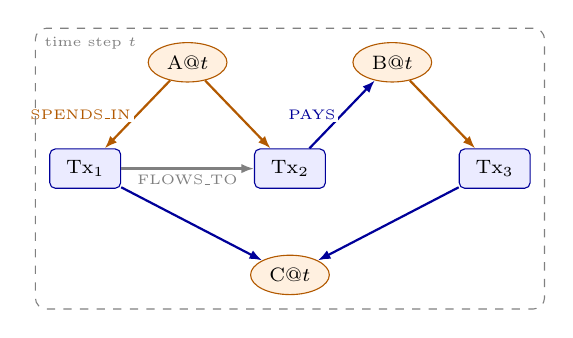
\begin{tikzpicture}[
  tx/.style={rectangle, rounded corners=2pt, draw=blue!60!black, fill=blue!8, minimum width=9mm, minimum height=5mm, font=\scriptsize},
  ad/.style={ellipse, draw=orange!70!black, fill=orange!12, minimum width=10mm, minimum height=5mm, inner sep=1pt, font=\scriptsize},
  rel/.style={-{Latex[length=1.6mm]}, thick},
  lab/.style={font=\tiny, fill=white, inner sep=1pt}]
\node[tx] (t1) at (0,0) {Tx$_1$};
\node[tx] (t2) at (2.6,0) {Tx$_2$};
\node[tx] (t3) at (5.2,0) {Tx$_3$};
\node[ad] (a1) at (1.3,1.35) {A@$t$};
\node[ad] (a2) at (3.9,1.35) {B@$t$};
\node[ad] (a3) at (2.6,-1.35) {C@$t$};
\draw[rel, gray] (t1) -- (t2) node[lab, midway, below=1pt] {FLOWS\_TO};
\draw[rel, orange!70!black] (a1) -- (t1) node[lab, midway, left=1pt] {SPENDS\_IN};
\draw[rel, orange!70!black] (a1) -- (t2);
\draw[rel, blue!60!black] (t2) -- (a2) node[lab, midway, left=1pt] {PAYS};
\draw[rel, orange!70!black] (a2) -- (t3);
\draw[rel, blue!60!black] (t1) -- (a3);
\draw[rel, blue!60!black] (t3) -- (a3);
\node[draw=gray, dashed, rounded corners, fit=(t1)(t3)(a1)(a2)(a3), inner sep=5pt] (box) {};
\node[font=\tiny, anchor=north west, gray] at (box.north west) {time step $t$};
\end{tikzpicture}
\caption{Time-sliced knowledge graph schema. Address nodes are instantiated per
time step; history enters only through causal node attributes. Two-hop paths
through an address define meta-relations: Tx$_1$ and Tx$_2$ are
\texttt{CO\_SPEND} (shared input A), Tx$_1$ and Tx$_3$ are
\texttt{CO\_RECEIVE} (shared output C), Tx$_2$ and Tx$_3$ are \texttt{CHAIN}
(Tx$_2$ pays B, which spends in Tx$_3$).}
\label{fig:schema}
\end{figure}

\subsection{Meta-relations and homophily}
Two-hop paths through an Address@t node define three meta-relations between
transactions: \texttt{CO\_SPEND} (a shared input address),
\texttt{CO\_RECEIVE} (a shared output address) and \texttt{CHAIN} (one
transaction pays an address that another spends from). Address instances
linked to more than 200 transactions in a step (67 exchange-like hubs) are
excluded from the meta-relations. Table~\ref{tab:homophily} reports, for
labelled transactions, the class-adjusted homophily~\cite{platonov2023}
(0 for random wiring, 1 for perfect homophily), together with the share of
illicit transactions that have at least one labelled neighbour (coverage) and
the share of their labelled neighbours that are illicit.

\begin{table}[t]
\caption{Label homophily of transaction relations (labelled nodes).}
\label{tab:homophily}
\centering
\footnotesize
\setlength{\tabcolsep}{3.2pt}
\resizebox{\columnwidth}{!}{%
\begin{tabular}{@{}lrrrrrr@{}}
\toprule
& \multicolumn{3}{c}{Train (steps 1--34)} & \multicolumn{3}{c}{Test (steps 35--49)} \\
\cmidrule(lr){2-4}\cmidrule(l){5-7}
Relation & Adj.\ hom. & Cov.\ & Ill.\ nbr & Adj.\ hom. & Cov.\ & Ill.\ nbr \\
\midrule
FLOWS\_TO   & 0.553 & 0.551 & 0.581 & 0.376 & 0.532 & 0.395 \\
CO\_SPEND$^{a}$ & 1.000 & 0.186 & 1.000 & 1.000 & 0.125 & 1.000 \\
CO\_RECEIVE & 1.000 & 0.759 & 1.000 & 1.000 & 0.667 & 1.000 \\
CHAIN       & 0.865 & 0.527 & 0.871 & 0.309 & 0.547 & 0.315 \\
KG union    & \textbf{0.954} & \textbf{0.906} & \textbf{0.957} & \textbf{0.915} & \textbf{0.930} & \textbf{0.921} \\
\bottomrule
\multicolumn{7}{@{}l}{\scriptsize Cov.: illicit transactions with a labelled neighbour. Ill.\ nbr: illicit share of}\\
\multicolumn{7}{@{}l}{\scriptsize their labelled neighbours. $^{a}$Homophilous by construction (labels follow inputs).}
\end{tabular}}
\end{table}

Three observations motivate graph learning on the TS-KG. First, the
transaction graph used by prior GNN work is only moderately homophilous and
becomes much less so after the dark-market shutdown in the test period
(adjusted homophily 0.55$\rightarrow$0.38), consistent with its weak results
under strict evaluation~\cite{maganti2026}. Second, the KG relations connect
93\% of illicit test transactions to labelled neighbours, of which 92\% are
illicit; this is the regime in which message passing is expected to
help~\cite{zhu2020,platonov2023}. Third, part of this signal follows directly
from how labels were made: transactions sharing an input address share the
labelling entity, so \texttt{CO\_SPEND} is perfectly homophilous by
construction. It covers only 13\% of illicit test transactions, however,
whereas \texttt{CO\_RECEIVE}, which is not determined by the labelling rule,
covers 67\%. In practice the shared output addresses are change addresses and
deposit addresses of the same entity, the structure that forensic address
clustering exploits~\cite{meiklejohn2013}. We return to this caveat in
Section~\ref{sec:discussion}.

\textbf{Address reuse across time is a licit signal.} Only 17 of the 1{,}083
illicit test transactions touch an address that was active during training,
against 5{,}833 of the 16{,}670 labelled test transactions overall. Illicit
actors use fresh addresses, so cross-period address knowledge mainly
identifies licit activity. Consequently, the \emph{unseen-entity} test view
recommended by~\cite{safar2026} (test transactions none of whose addresses
appeared in training) retains 98\% of the illicit test transactions.

\section{Experimental Design}\label{sec:method}

\textbf{Research questions.}
\textbf{RQ1:} once feature leakage and evaluation protocol are controlled, does
knowledge-graph enrichment improve illicit-transaction detection, and does
message passing over the KG beat tree ensembles given the same knowledge?
\textbf{RQ2:} which class-imbalance strategy gives the best precision--recall
trade-off? \textbf{RQ3:} which features drive predictions, and do model
families agree? \textbf{RQ4:} what does each approach cost to train on a
CPU-only budget?

\textbf{Tabular KG features.} To separate the value of KG \emph{knowledge}
from the value of \emph{message passing}, we derive 15 causal features per
transaction from the TS-KG: for input and output addresses separately, the
number of addresses, the share and mean count of earlier appearances, the
maximum address age and the number of hubs; the degree of the transaction
under each relation (\texttt{FLOWS\_TO}, \texttt{CO\_SPEND},
\texttt{CO\_RECEIVE}, \texttt{CHAIN}); and the size of its connected
component in the step-local transaction--address graph (an entity-cluster
proxy). A further variant (\textsc{+Nbr}) adds the mean \textsc{Clean}
features of each transaction's KG neighbours, a hand-crafted one-hop
aggregation that uses no labels.

\textbf{Models.} Tree ensembles: logistic regression (LR), RF~\cite{breiman2001}
(500 trees, balanced class weights) and XGBoost~\cite{chen2016} (depth 6,
learning rate 0.05, up to 1{,}000 rounds with early stopping on validation
PR-AUC, positive-class weight equal to the training imbalance ratio). Graph
models: a relational GraphSAGE~\cite{hamilton2017,schlichtkrull2018}
(\textsc{KG-SAGE}) with one mean-aggregation weight matrix per relation and
direction, two layers of width 64, and jumping-knowledge concatenation into a
two-layer classifier; \textsc{SAGE-Flow}, the same model restricted to
\texttt{FLOWS\_TO} edges as in prior work; and an \textsc{MLP} of matched
capacity with no edges. All graph models receive \emph{exactly} the inputs of
the \textsc{Clean+KG} trees (\textsc{Clean} plus the 15 KG features), so the
comparison isolates message passing. Address instances linked to a single
transaction cannot connect transactions and are already summarised by the KG
features; they are pruned from the graph (246{,}545 instances remain). Graph
models are trained full-batch with Adam (weight decay $5\times10^{-4}$,
dropout 0.3 on transaction representations) and class-weighted binary
cross-entropy for up to 300 epochs, keeping the epoch with the best
validation PR-AUC (patience 40). For each neural model the learning rate is
selected from $\{10^{-3}, 5\times10^{-3}\}$ by mean validation PR-AUC over
two tuning seeds that are disjoint from the evaluation seeds; all three
selected $5\times10^{-3}$.

\textbf{Ablations.} \textsc{KG-SAGE} without \texttt{FLOWS\_TO}, without
input (\texttt{SPENDS\_IN}) and without output (\texttt{PAYS}) relations,
and with address--transaction edges randomly rewired within each step (which
destroys entity structure but preserves each transaction's number of
addresses), following the edge-shuffle test of~\cite{maganti2026}.

\textbf{Metrics.} The positive class is illicit. We report illicit-class F1,
precision and recall at the threshold that maximises F1 on the validation
window, threshold-free PR-AUC (average precision) and ROC-AUC, and precision
among the 1\% highest-scored transactions (an analyst's review budget).
Accuracy is not reported because predicting ``licit'' everywhere already scores
93.5\% on the test set~\cite{he2009}. Results are means $\pm$ standard
deviations over five seeds (two for graph ablations, three for imbalance
strategies). We report the full test window, the unseen-entity view, and the
periods before and after the dark-market shutdown at step
43~\cite{weber2019}.

\textbf{Imbalance strategies (RQ2).} For RF and XGBoost on \textsc{Clean+KG}:
no correction, class weighting, SMOTE~\cite{chawla2002} and
SMOTE-ENN~\cite{batista2004} applied to the training window only, each at the
default 0.5 threshold and at the validation-tuned threshold.

\textbf{Explanations (RQ3).} TreeSHAP~\cite{lundberg2017} for XGBoost on
\textsc{All} and \textsc{Clean+KG}; gradient$\times$input attributions for
\textsc{KG-SAGE} on the same inputs; agreement measured by Spearman rank
correlation and top-10 overlap of feature importances.

\textbf{Implementation.} Python 3.12, scikit-learn, XGBoost, PyTorch 2.15 and
PyTorch Geometric 2.8 on a laptop CPU (8 threads, 14\,GB RAM, no GPU).
Seeds fix all random choices, but multithreaded CPU arithmetic is not
bit-exact, so graph-model results can differ slightly with the thread count.

\section{Results}\label{sec:results}

\begin{table*}[t]
\caption{Illicit-class results on the test period (steps 35--49), mean $\pm$ std over seeds. Thresholds are tuned on the validation window. Best leakage-controlled value in bold.}
\label{tab:main}
\centering
\footnotesize
\begin{tabular}{@{}llccccccr@{}}
\toprule
Model & Features & F1 & Precision & Recall & PR-AUC & ROC-AUC & P@1\% & Fit (s) \\
\midrule
\multicolumn{9}{@{}l}{\textit{Leaky features (as in prior work)}} \\
RF & All & 0.799\,$\pm$\,0.007 & 0.902\,$\pm$\,0.020 & 0.717\,$\pm$\,0.003 & 0.788\,$\pm$\,0.001 & 0.927\,$\pm$\,0.002 & 1.000\,$\pm$\,0.000 & 28 \\
XGB & All & 0.803\,$\pm$\,0.004 & 0.902\,$\pm$\,0.012 & 0.724\,$\pm$\,0.002 & 0.796\,$\pm$\,0.002 & 0.928\,$\pm$\,0.004 & 1.000\,$\pm$\,0.000 & 24 \\
\multicolumn{9}{@{}l}{\textit{Leakage-controlled features}} \\
LR & Clean & 0.383 & 0.298 & 0.537 & 0.204 & 0.822 & 0.024 & 5 \\
RF & Clean & 0.561\,$\pm$\,0.006 & 0.635\,$\pm$\,0.021 & 0.504\,$\pm$\,0.005 & 0.572\,$\pm$\,0.002 & 0.863\,$\pm$\,0.003 & 0.951\,$\pm$\,0.003 & 25 \\
XGB & Clean & 0.561\,$\pm$\,0.012 & 0.630\,$\pm$\,0.042 & 0.506\,$\pm$\,0.011 & 0.608\,$\pm$\,0.013 & 0.892\,$\pm$\,0.008 & 0.963\,$\pm$\,0.020 & 6 \\
\multicolumn{9}{@{}l}{\textit{+ knowledge-graph features}} \\
RF & Clean+KG & 0.604\,$\pm$\,0.009 & 0.681\,$\pm$\,0.035 & 0.543\,$\pm$\,0.007 & 0.623\,$\pm$\,0.004 & 0.871\,$\pm$\,0.007 & 0.994\,$\pm$\,0.000 & 23 \\
XGB & Clean+KG & \textbf{0.651\,$\pm$\,0.004} & 0.821\,$\pm$\,0.016 & 0.540\,$\pm$\,0.007 & \textbf{0.683\,$\pm$\,0.007} & \textbf{0.905\,$\pm$\,0.004} & \textbf{1.000\,$\pm$\,0.000} & 20 \\
RF & Clean+KG+Nbr & 0.615\,$\pm$\,0.028 & 0.648\,$\pm$\,0.071 & 0.589\,$\pm$\,0.006 & 0.677\,$\pm$\,0.003 & 0.899\,$\pm$\,0.005 & 0.996\,$\pm$\,0.003 & 115 \\
XGB & Clean+KG+Nbr & 0.556\,$\pm$\,0.119 & 0.527\,$\pm$\,0.183 & 0.617\,$\pm$\,0.015 & 0.668\,$\pm$\,0.075 & 0.880\,$\pm$\,0.064 & 0.992\,$\pm$\,0.012 & 67 \\
\multicolumn{9}{@{}l}{\textit{Neural models (inputs = Clean+KG)}} \\
MLP & Clean+KG & 0.500\,$\pm$\,0.058 & 0.513\,$\pm$\,0.168 & 0.529\,$\pm$\,0.082 & 0.526\,$\pm$\,0.101 & 0.884\,$\pm$\,0.009 & 0.838\,$\pm$\,0.224 & 43 \\
SAGE-Flow & Clean+KG & 0.461\,$\pm$\,0.051 & 0.485\,$\pm$\,0.077 & 0.445\,$\pm$\,0.051 & 0.359\,$\pm$\,0.056 & 0.863\,$\pm$\,0.019 & 0.508\,$\pm$\,0.137 & 306 \\
KG-SAGE & Clean+KG & 0.376\,$\pm$\,0.036 & 0.276\,$\pm$\,0.033 & 0.601\,$\pm$\,0.082 & 0.227\,$\pm$\,0.052 & 0.838\,$\pm$\,0.018 & 0.147\,$\pm$\,0.148 & 511 \\
\bottomrule
\end{tabular}
\end{table*}

\subsection{Feature leakage inflates the benchmark}
Table~\ref{tab:main} first reproduces the literature: with \textsc{All}
features, RF and XGBoost reach illicit F1 of about 0.80 and PR-AUC of about 0.79,
in line with the strongest leakage-controlled baselines reported
before~\cite{maganti2026,ichull2026twin}. Removing the address statistics
computed after the test period and the successor aggregates
(\textsc{Clean}) lowers F1 by about 0.24 and PR-AUC by 0.19--0.22 for both
ensembles. A large part of the apparent skill on this benchmark therefore
comes from information that is not available when a transaction must be
scored, confirming the audit of~\cite{safar2026} quantitatively at the
transaction level, in the same direction as the address-level drop reported
in~\cite{liang2026}. The leaky models also score almost identically on the
unseen-entity view (Table~\ref{tab:views}): because illicit actors rarely
reuse addresses across periods (Section~\ref{sec:kg}), the leakage here acts
through \emph{future} address statistics rather than through memorised
entities.

\subsection{Knowledge-graph knowledge recovers part of the gap}
Adding the 15 causal TS-KG features raises XGBoost from F1
\XgbCleanFone{} to \XgbCleanKgFone{} and PR-AUC
from \XgbCleanPr{} to \XgbCleanKgPr{},
with seed-to-seed standard deviations below 0.01; RF improves by a smaller
margin. Information about the addresses a transaction touches is thus genuinely
useful, provided it is computed causally. Adding hand-crafted one-hop
aggregates over the KG (\textsc{+Nbr}) further improves ranking for RF
(PR-AUC \RfCleanKgNbrPr{}, and \RfCleanKgNbrUnseenPr{} on unseen entities) but
makes thresholded alerts less stable: XGBoost becomes sensitive to the seed,
and most additional false alarms fall on recurring licit transactions that
have no KG neighbours, whose scores shift between the validation and test
periods. The compact structural features are the more robust choice.

\subsection{Message passing over the knowledge graph}
The neural models receive exactly the \textsc{Clean+KG} inputs of the
trees, so differences between them isolate message passing. On the
validation window KG-SAGE is the strongest leakage-controlled model (mean
validation PR-AUC \KgSageValPr{}, against \XgbCleanKgValPr{} for XGBoost on
the same features). On the full test period, however, it is the weakest
(F1 \KgSageFone{}, PR-AUC \KgSagePr{}), below the MLP (\MlpPr{}), SAGE-Flow
(\SageFlowPr{}) and XGBoost (\XgbCleanKgPr{}). The unseen-entity view
(Table~\ref{tab:views}) locates the failure. On transactions of entities
that never appeared in training, KG-SAGE reaches PR-AUC
\KgSageUnseenPr{}, clearly above the MLP (\MlpUnseenPr{}) and SAGE-Flow
(\SageFlowUnseenPr{}): message passing over the KG does help to recognise new
entities, although it still trails XGBoost (\XgbCleanKgUnseenPr{}). The
collapse comes from \emph{recurring} licit entities, mostly exchange-like
clusters active since the training period: \DiagFpRecurShare{} of the
\DiagFp{} false alarms of the seed-0 model fall on them, and their false-alarm
rate is \DiagFpRateRecur{} against \DiagFpRateUnseen{} for licit transactions of
new entities. These alarms are not explained by inputs outside the training
range (\DiagOorFp{} of the falsely flagged recurring transactions touch an
address node with an out-of-range attribute, against \DiagOorTn{} of the
correctly cleared ones), so they reflect a change in the relational
neighbourhoods of long-lived licit entities rather than extrapolation. Thus,
even on a highly homophilous graph, learned message passing over entity
structure is fragile under temporal shift, whereas the same knowledge,
summarised as a handful of causal features and consumed by a tree ensemble,
transfers.

\begin{table}[t]
\caption{KG-SAGE relation ablations (test period; mean $\pm$ std over the two ablation seeds).}
\label{tab:ablation}
\centering
\footnotesize
\setlength{\tabcolsep}{4pt}
\resizebox{\columnwidth}{!}{%
\begin{tabular}{@{}lcccc@{}}
\toprule
& \multicolumn{3}{c}{All test} & Unseen \\
\cmidrule(lr){2-4}\cmidrule(l){5-5}
Graph & F1 & PR-AUC & $\Delta$PR-AUC & PR-AUC \\
\midrule
Full TS-KG & 0.376\,$\pm$\,0.019 & 0.195\,$\pm$\,0.025 & -- & 0.672 \\
-- FLOWS\_TO & 0.386\,$\pm$\,0.138 & 0.237\,$\pm$\,0.140 & +0.042 & 0.596 \\
-- SPENDS\_IN (inputs) & 0.391\,$\pm$\,0.037 & 0.210\,$\pm$\,0.030 & +0.015 & 0.604 \\
-- PAYS (outputs) & 0.412\,$\pm$\,0.133 & 0.295\,$\pm$\,0.178 & +0.100 & 0.544 \\
Address edges rewired & 0.519\,$\pm$\,0.043 & 0.471\,$\pm$\,0.070 & +0.276 & 0.556 \\
FLOWS\_TO only & 0.416\,$\pm$\,0.012 & 0.311\,$\pm$\,0.054 & +0.116 & 0.499 \\
No edges (MLP) & 0.496\,$\pm$\,0.047 & 0.563\,$\pm$\,0.074 & +0.368 & 0.572 \\
\bottomrule
\end{tabular}}
\end{table}

The relation ablations (Table~\ref{tab:ablation}) show the two sides of this
behaviour. On unseen entities, the full TS-KG gives the best KG-SAGE PR-AUC
(\AblFullUnseenPr{} over the ablation seeds); removing any relation lowers it,
most of all removing the output relation (\AblNoOutUnseenPr{}), and randomly
rewiring the address--transaction edges within each step lowers it to
\AblShufUnseenPr{}, below the edge-free MLP. The real entity structure is
therefore what helps the model recognise new entities. On the full test
period, the same interventions have the opposite effect: removing relations
improves PR-AUC, and rewiring raises it from \AblFullPr{} to \AblShufPr{}. As
in the edge-shuffle test of~\cite{maganti2026}, real structure can hurt; the
KG view adds that it hurts specifically through the neighbourhoods of
recurring licit entities, while it helps for new ones.

\subsection{Temporal drift and evaluation views}
\begin{table}[t]
\caption{Illicit F1 by evaluation view (mean over seeds).}
\label{tab:views}
\centering
\footnotesize
\setlength{\tabcolsep}{3.5pt}
\resizebox{\columnwidth}{!}{%
\begin{tabular}{@{}lcccc@{}}
\toprule
Model & All test & Unseen entities & Steps 35--42 & Steps 43--49 \\
\midrule
XGB, All & 0.803 & 0.808 & 0.898 & 0.035 \\
XGB, Clean & 0.561 & 0.591 & 0.672 & 0.026 \\
XGB, Clean+KG & 0.651 & 0.658 & 0.740 & 0.014 \\
SAGE-Flow & 0.461 & 0.562 & 0.541 & 0.021 \\
KG-SAGE & 0.376 & 0.629 & 0.443 & 0.028 \\
\midrule
\# illicit & 1083 & 1066 & 914 & 169 \\
\bottomrule
\end{tabular}}
\end{table}
Fig.~\ref{fig:perstep} and Table~\ref{tab:views} show that every model,
leaky or not, collapses after the dark-market shutdown at step
43~\cite{weber2019}: illicit F1 over steps 43--49 is below 0.07 for all models,
because the few illicit transactions that remain differ from those seen in
training and the illicit base rate falls sharply~\cite{maganti2026}. Before
the shutdown the differences between feature sets and models are large and
consistent. Averaged metrics over the whole test period therefore mostly
measure the first eight test steps, and per-step reporting is essential.

\begin{figure}[t]
\centering
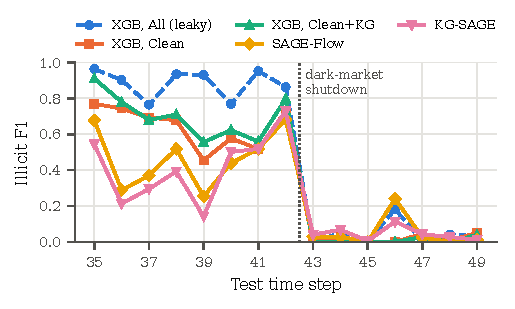
\includegraphics[width=\columnwidth]{figures/fig_per_step.pdf}
\caption{Illicit F1 per test time step (mean over seeds). All models collapse
after the dark-market shutdown at step 43.}
\label{fig:perstep}
\end{figure}

\subsection{Class imbalance (RQ2)}
\begin{table}[t]
\caption{Imbalance strategies on Clean+KG features (test F1; three seeds). PR-AUC does not depend on the threshold.}
\label{tab:imbalance}
\centering
\footnotesize
\setlength{\tabcolsep}{3pt}
\begin{tabular}{@{}llccc@{}}
\toprule
Model & Strategy & F1 @0.5 & F1 @val & PR-AUC \\
\midrule
XGB & None & 0.214\,$\pm$\,0.371 & 0.563\,$\pm$\,0.076 & 0.583\,$\pm$\,0.076 \\
XGB & Class weights & 0.609\,$\pm$\,0.010 & 0.652\,$\pm$\,0.003 & 0.684\,$\pm$\,0.005 \\
XGB & SMOTE & 0.623\,$\pm$\,0.012 & 0.640\,$\pm$\,0.009 & 0.683\,$\pm$\,0.004 \\
XGB & SMOTE-ENN & 0.573\,$\pm$\,0.008 & 0.658\,$\pm$\,0.006 & 0.701\,$\pm$\,0.006 \\
\midrule
RF & None & 0.594\,$\pm$\,0.003 & 0.499\,$\pm$\,0.071 & 0.598\,$\pm$\,0.002 \\
RF & Class weights & 0.616\,$\pm$\,0.003 & 0.603\,$\pm$\,0.010 & 0.624\,$\pm$\,0.003 \\
RF & SMOTE & 0.622\,$\pm$\,0.003 & 0.608\,$\pm$\,0.012 & 0.642\,$\pm$\,0.004 \\
RF & SMOTE-ENN & 0.595\,$\pm$\,0.005 & 0.616\,$\pm$\,0.004 & 0.650\,$\pm$\,0.003 \\
\bottomrule
\end{tabular}
\end{table}
Table~\ref{tab:imbalance} shows that some correction for imbalance is
essential: an uncorrected XGBoost model at the default threshold collapses on
some seeds (F1 $0.21\pm0.37$). With correction, the strategies are close.
For XGBoost, class weighting and SMOTE-ENN with a validation-tuned threshold
are statistically tied (F1 0.652 and 0.658), and SMOTE-ENN gives the highest
PR-AUC (0.701). For RF, all corrections reach F1 0.60--0.62. Tuning the
threshold on the validation window matters more than the choice of
resampling method for XGBoost, while for RF the default threshold is already
adequate once classes are re-weighted. Oversampling cannot be applied to the
graph models, so class weighting with threshold tuning is the strategy that
transfers across both families.

\subsection{Explanations (RQ3)}
\begin{figure}[t]
\centering
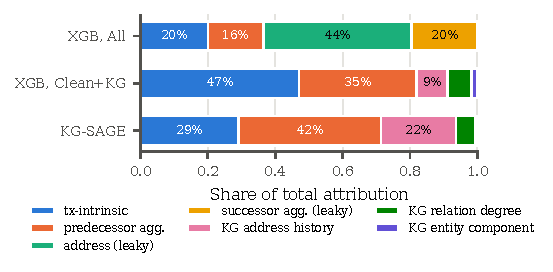
\includegraphics[width=\columnwidth]{figures/fig_attribution.pdf}
\caption{Share of total attribution per feature group: TreeSHAP for XGBoost,
gradient$\times$input for KG-SAGE (test period, seed 0).}
\label{fig:attr}
\end{figure}
Fig.~\ref{fig:attr} makes the leakage visible: XGBoost trained on
\textsc{All} features places \ShapAllLeaky{} of its attribution on the leaky
groups, \ShapAllAddr{} on address statistics computed after the test period
alone. With \textsc{Clean+KG} inputs, the KG features receive \ShapCleanKgKg{}
of the XGBoost attribution, led by the \texttt{CO\_RECEIVE} degree and the age
of the input addresses, while the transaction's own size, fee and value
statistics remain the strongest signals. KG-SAGE relies more on the graph
(\GxiKg{} of its attribution), above all on address history
(\GxiAddrHist{}, against \ShapCleanKgAddrHist{} for XGBoost). The two families
agree only moderately (Spearman $\rho=\ExplainRho$ over all features,
\ExplainOverlap{} of the top-10 features shared). Because address age and
reuse change systematically over time, the stronger reliance of the graph
model on address history is consistent with its weaker transfer to the test
period. Feature names remain those of the dataset; the semantics recovered
in~\cite{safar2026} make them interpretable (\eg\ Local~1--21 are value, fee
and input/output statistics).

\subsection{Computational cost (RQ4)}
All experiments ran on a laptop CPU. Tree ensembles on \textsc{Clean+KG}
features train in about \XgbCleanKgFit{}\,s (XGBoost) and \RfCleanKgFit{}\,s
(RF); building the TS-KG and its 15 features takes under five seconds. The graph
models are one to two orders of magnitude more expensive: \MlpFit{}\,s for the
MLP, \SageFlowFit{}\,s for SAGE-Flow and \KgSageFit{}\,s for KG-SAGE per run,
after pruning single-transaction address instances and replacing generic
scatter operations with sparse matrix products, without which a KG-SAGE epoch
took about 18\,s. Under a CPU budget, one of the cheapest models is also the most
accurate leakage-controlled one.

\section{Discussion}\label{sec:discussion}

\textbf{When does graph learning help?} Our results separate three claims
that are usually conflated. (1) \emph{Graph structure carries signal}: yes.
The TS-KG relations are far more homophilous than the transaction graph
(Table~\ref{tab:homophily}), and causal KG features add
\XgbKgGain{} in F1 to XGBoost
(Table~\ref{tab:main}). The motivation for graph methods on this problem is
therefore real, but it lies in the \emph{entity} structure that a knowledge
graph exposes, not in the transaction-to-transaction graph used by prior GNN
work. (2) \emph{Message passing exploits it}: only partly. On transactions of new
entities, KG-SAGE clearly improves over a graph-free network and over message
passing on the transaction graph, so learning over the KG does capture entity
signal; but it never matches a tree ensemble given the same knowledge, and it
raises many false alarms on recurring licit entities whose neighbourhoods
change over time. High homophily on the training graph is therefore not
sufficient for a GNN advantage under distribution shift, which refines the
conditions conjectured in~\cite{maganti2026}. (3) \emph{Prior reports of
strong performance}: largely a consequence of leaked features, which account for
\XgbLeakDrop{} of the \XgbAllFone{} F1 of XGBoost (\XgbLeakShare{}). For
practitioners, the actionable recommendation is to build the entity knowledge
graph, compute causal features from it, and give them to a well-regularised
tree ensemble with class weights and a validation-tuned threshold; graph
neural networks should be evaluated over several later periods, because a
single validation window can be badly misleading.

\textbf{Label provenance.} Elliptic labels are assigned per controlling
entity of the input addresses~\cite{weber2019,safar2026}. The perfect
homophily of \texttt{CO\_SPEND} is therefore partly a property of the
labelling rule, and the near-perfect homophily of \texttt{CO\_RECEIVE}
suggests that shared output addresses mostly connect transactions of the same
entity (change and deposit addresses). A KG that makes entity structure
explicit thus aligns the model with the structure that defines the labels.
This is also how investigations work in practice, since attributing addresses
to entities is the basis of Bitcoin forensics~\cite{meiklejohn2013}, but it
means that gains measured on Elliptic partly reflect entity re-identification
\emph{within} a time step. Labels produced by a different process, or
entity-disjoint evaluation within a step, may show smaller gains. Because
illicit actors almost never reuse addresses across periods, the
cross-period form of this problem (memorising known entities) is negligible
here, as the unseen-entity view confirms.

\textbf{Threats to validity.} (i) A single dataset, two years of Bitcoin
activity ending in 2017, before SegWit-heavy and Taproot usage. (ii) The
within-step observation assumption: features and edges of a time step are
used to score transactions of that step, i.e.\ scoring happens at the end of
each step; real-time scoring would see fewer neighbours. (iii) The released
Elliptic++ edges cover only transactions inside the benchmark, so address
histories are truncated to the sampled transactions rather than the full
ledger~\cite{safar2026}. (iv) Hyperparameter search was limited by a CPU-only
budget: tree ensembles use standard settings with early stopping, and the
graph models select only the learning rate on the validation window; wider
searches could change the size of the gaps, though not the leakage effect,
which exceeds every other difference we observe. (v) An earlier version of
the \textsc{+Nbr} features encoded transactions without KG neighbours as zero,
which in z-scored space is a valid value; this produced false alarms on
isolated licit transactions and was corrected by encoding them as missing.
All reported numbers use the corrected features.

\section{Conclusion}\label{sec:conclusion}

We asked when graph learning helps to detect illicit Bitcoin transactions once
evaluation is free of leakage. Building a time-sliced transaction--address
knowledge graph from Elliptic++ showed that the graph signal is real but lives
in entity structure: KG relations are far more homophilous than the
transaction graph, and causal KG features improve a leakage-controlled
XGBoost from F1 \XgbCleanFone{} to \XgbCleanKgFone{}. Relational message
passing over the same graph excels on the validation window and helps on new
entities, but misfires on recurring licit entities in later periods, and all
models collapse after the dark-market shutdown. At the same time, \XgbLeakShare{} of the F1 reported for standard
baselines comes from features that are only observable after the test period.
Future work should (i) evaluate on an entity-disjoint benchmark built from
the full ledger with time-scoped features~\cite{safar2026}, (ii) test whether
temporal or continually retrained GNNs close the validation--test gap, and
(iii) extend the knowledge graph with off-chain entity attributions and other
chains.

\section*{Code and Data Availability}
Code, configuration and all result files are available at
\url{https://github.com/TahaNaqv/kg-bitcoin-aml}. Elliptic++ is available from
its authors~\cite{elmougy2023}; the data are not redistributed because of the
Elliptic licence (CC BY-NC-ND 4.0).

\section*{Ethics Statement}
The data are public, pseudonymous blockchain records without personal
information. Labels reflect third-party investigative judgements and may be
noisy or biased; model outputs are decision support for analysts, not
evidence of wrongdoing by any individual or entity.


\begin{thebibliography}{00}
\footnotesize

\bibitem{chainalysis2026} Chainalysis, ``The 2026 Crypto Crime Report,'' Chainalysis Inc., New York, NY, USA, 2026.

\bibitem{weber2019} M.~Weber, G.~Domeniconi, J.~Chen, D.~K.~I. Weidele, C.~Bellei, T.~Robinson, and C.~E. Leiserson, ``Anti-money laundering in Bitcoin: Experimenting with graph convolutional networks for financial forensics,'' in \emph{Proc. KDD Workshop on Anomaly Detection in Finance}, 2019, arXiv:1908.02591.

\bibitem{elmougy2023} Y.~Elmougy and L.~Liu, ``Demystifying fraudulent transactions and illicit nodes in the Bitcoin network for financial forensics,'' in \emph{Proc. 29th ACM SIGKDD Conf. Knowledge Discovery and Data Mining (KDD)}, 2023, pp.~5244--5254.

\bibitem{maganti2026} S.~Maganti, ``When graph structure becomes a liability: A critical re-evaluation of graph neural networks for Bitcoin fraud detection under temporal distribution shift,'' 2026, arXiv:2604.19514.

\bibitem{ichull2026twin} A.~P. Ichull and J.~C. Sopuru, ``TWIN-GNN: An interpretable multi-graph framework for illicit Bitcoin transaction and wallet detection,'' \emph{J. Cybersecurity and Privacy}, vol.~6, no.~6, p.~186, 2026.

\bibitem{safar2026} M.~{\v S}af{\'a}{\v r}, J.~Pluskal, V.~Vesel{\'y}, and O.~Ry{\v s}av{\'y}, ``The enemy of reproducibility is opacity: What's inside the Elliptic Bitcoin dataset (and why it is wrong),'' \emph{Forensic Science International: Digital Investigation}, vol.~57, p.~302124, 2026 (DFRWS USA 2026).

\bibitem{meiklejohn2013} S.~Meiklejohn, M.~Pomarole, G.~Jordan, K.~Levchenko, D.~McCoy, G.~M. Voelker, and S.~Savage, ``A fistful of bitcoins: Characterizing payments among men with no names,'' in \emph{Proc. ACM Internet Measurement Conf. (IMC)}, 2013, pp.~127--140.

\bibitem{kipf2017} T.~N. Kipf and M.~Welling, ``Semi-supervised classification with graph convolutional networks,'' in \emph{Proc. Int. Conf. Learning Representations (ICLR)}, 2017.

\bibitem{asiri2025} A.~Asiri and K.~Somasundaram, ``Graph convolution network for fraud detection in Bitcoin transactions,'' \emph{Scientific Reports}, vol.~15, p.~11076, 2025.

\bibitem{zheng2025} Z.~Zheng, B.~Zhou, and Y.~Song, ``Temporal-aware graph attention network for cryptocurrency transaction fraud detection,'' 2025, arXiv:2506.21382.

\bibitem{lin2026} Z.~Lin, Q.~Luo, D.~Wu, J.~Shen, L.~Li, X.~Nong, and Z.~Qin, ``Detecting illicit transactions in Bitcoin: A wavelet-temporal graph transformer approach for anti-money laundering,'' \emph{Scientific Reports}, vol.~16, p.~1548, 2026.

\bibitem{ferretti2024} S.~Ferretti, G.~D'Angelo, and V.~Ghini, ``On the use of heterogeneous graph neural networks for detecting malicious activities: A case study with cryptocurrencies,'' in \emph{Proc. OASIS '24}, Poznan, Poland, 2024, pp.~33--40.

\bibitem{perezcano2025} V.~P{\'e}rez-Cano and F.~Jurado, ``Fraud detection in cryptocurrency networks---An exploration using anomaly detection and heterogeneous graph transformers,'' \emph{Future Internet}, vol.~17, no.~1, p.~44, 2025.

\bibitem{he2009} H.~He and E.~A. Garcia, ``Learning from imbalanced data,'' \emph{IEEE Trans. Knowl. Data Eng.}, vol.~21, no.~9, pp.~1263--1284, 2009.

\bibitem{liang2026} R.~Liang, S.~Trimborn, and N.~van Giersbergen, ``Revisiting Elliptic++ for Bitcoin forensics: Feature reconstruction and leakage-resistant evaluation,'' 2026, arXiv:2611.04000.

\bibitem{malik2026} A.~Malik, ``Do transaction-level and actor-level AML queues agree? An empirical evaluation of granularity effects on the Elliptic++ graph,'' 2026, arXiv:2604.23494.

\bibitem{hogan2021} A.~Hogan \emph{et~al.}, ``Knowledge graphs,'' \emph{ACM Computing Surveys}, vol.~54, no.~4, pp.~71:1--71:37, 2021.

\bibitem{ugarterojas2020} H.~Ugarte-Rojas and B.~Chullo-Llave, ``BLONDiE: Blockchain ontology with dynamic extensibility,'' 2020, arXiv:2008.09518.

\bibitem{jia2025kgbert4eth} Y.~Jia, Y.~Tian, L.~Zhang, Y.~Wang, J.~Sun, and L.~Song, ``KGBERT4Eth: A feature-complete transformer powered by knowledge graph for multi-task Ethereum fraud detection,'' 2025, arXiv:2509.03860.

\bibitem{schlichtkrull2018} M.~Schlichtkrull, T.~N. Kipf, P.~Bloem, R.~van~den Berg, I.~Titov, and M.~Welling, ``Modeling relational data with graph convolutional networks,'' in \emph{Proc. Extended Semantic Web Conf. (ESWC)}, 2018, pp.~593--607.

\bibitem{hamilton2017} W.~L. Hamilton, R.~Ying, and J.~Leskovec, ``Inductive representation learning on large graphs,'' in \emph{Advances in Neural Information Processing Systems (NeurIPS)}, 2017, pp.~1024--1034.

\bibitem{zhu2020} J.~Zhu, Y.~Yan, L.~Zhao, M.~Heimann, L.~Akoglu, and D.~Koutra, ``Beyond homophily in graph neural networks: Current limitations and effective designs,'' in \emph{Advances in Neural Information Processing Systems (NeurIPS)}, 2020, pp.~7793--7804.

\bibitem{platonov2023} O.~Platonov, D.~Kuznedelev, A.~Babenko, and L.~Prokhorenkova, ``Characterizing graph datasets for node classification: Homophily-heterophily dichotomy and beyond,'' in \emph{Advances in Neural Information Processing Systems (NeurIPS)}, 2023.

\bibitem{chen2016} T.~Chen and C.~Guestrin, ``XGBoost: A scalable tree boosting system,'' in \emph{Proc. ACM SIGKDD Int. Conf. Knowledge Discovery and Data Mining}, 2016, pp.~785--794.

\bibitem{chawla2002} N.~V. Chawla, K.~W. Bowyer, L.~O. Hall, and W.~P. Kegelmeyer, ``SMOTE: Synthetic minority over-sampling technique,'' \emph{J. Artificial Intelligence Research}, vol.~16, pp.~321--357, 2002.

\bibitem{batista2004} G.~E. Batista, R.~C. Prati, and M.~C. Monard, ``A study of the behavior of several methods for balancing machine learning training data,'' \emph{ACM SIGKDD Explorations Newsletter}, vol.~6, no.~1, pp.~20--29, 2004.

\bibitem{lundberg2017} S.~M. Lundberg and S.-I. Lee, ``A unified approach to interpreting model predictions,'' in \emph{Advances in Neural Information Processing Systems (NeurIPS)}, 2017, pp.~4765--4774.

\bibitem{taher2024} S.~Taher, S.~Ameen, and J.~Ahmed, ``Advanced fraud detection in blockchain transactions: An ensemble learning and explainable AI approach,'' \emph{Engineering, Technology \& Applied Science Research}, vol.~14, pp.~12822--12830, 2024.

\bibitem{chithanuru2025} V.~Chithanuru and M.~Ramaiah, ``Proactive detection of anomalous behavior in Ethereum accounts using XAI-enabled ensemble stacking with Bayesian optimization,'' \emph{PeerJ Computer Science}, vol.~11, p.~e2630, 2025.

\bibitem{kaufman2012} S.~Kaufman, S.~Rosset, C.~Perlich, and O.~Stitelman, ``Leakage in data mining: Formulation, detection, and avoidance,'' \emph{ACM Trans. Knowl. Discov. Data}, vol.~6, no.~4, pp.~1--21, 2012.

\bibitem{kapoor2023} S.~Kapoor and A.~Narayanan, ``Leakage and the reproducibility crisis in machine-learning-based science,'' \emph{Patterns}, vol.~4, no.~9, p.~100804, 2023.

\bibitem{breiman2001} L.~Breiman, ``Random forests,'' \emph{Machine Learning}, vol.~45, pp.~5--32, 2001.

\end{thebibliography}


\end{document}
